%%for slideshow
\documentclass[ignorenonframetext]{beamer} %add option 'draft' for quicker compilation
\usepackage{amsmath,amssymb,multirow}
\newcommand{\slides}{1}
%this only compiles frames with [label=current]
%\includeonlyframes{current} 
 
%for handouts
%\documentclass[a4paper,12pt]{article}
%\usepackage{beamerarticle}
%\newcommand{\slides}{0}

\mode<presentation>{
% for theme info see:
% http://www.ctan.org/tex-archive/macros/latex/contrib/beamer/doc/beameruserguide.pdf
\usetheme{default}
  \setbeamercovered{transparent}
  %Add university logo
  %\pgfdeclareimage[height=1cm]{university-logo}{logo}
  %\logo{\pgfuseimage{university-logo}}
  % If you wish to uncover everything in a step-wise fashion, uncomment
  % the following command:
%  \beamerdefaultoverlayspecification{<+->}

% get rid of navigation panel
\setbeamertemplate{navigation symbols}{} 

	\newcommand{\tcr}{\textcolor{red}}
}
\mode<article>{
  \usepackage{fullpage}
	\newcommand{\tcr}{\textcolor{black}}
  \renewcommand{\baselinestretch}{1.0}
  \oddsidemargin -1.5cm \evensidemargin -1.5in
  \topmargin=-1.5cm \headheight=0pt
  \headsep 0pt \textwidth=19cm
  \textheight=27cm \columnsep 10pt \columnseprule 0pt \parindent 0pt
  \parskip 0.0pt
  \usepackage{tweaklist}
  \renewcommand{\itemhook}{
    \setlength{\topsep}{-0pt}
    \setlength{\itemsep}{-0pt}
    \setlength{\parsep}{-0pt}
  }
  \renewcommand{\enumhook}{
    \setlength{\topsep}{-0pt}
    \setlength{\itemsep}{-0pt}
    \setlength{\parsep}{-0pt}
  }
}

\usepackage[english]{babel}
\usepackage[latin1]{inputenc}
\usepackage{helvet}
\renewcommand*\familydefault{\sfdefault} %% Only if the base font of the document is to be sans serif
%\usepackage{times}
\usepackage[T1]{fontenc}
\usepackage{graphics,graphicx,fancyhdr,color,amsmath,url,enumerate,alltt}
\usepackage{epsf}
\usepackage{ifthen}


\newcommand{\bc}{\begin{center}}
\newcommand{\ec}{\end{center}}
\newcommand{\bn}{\begin{enumerate}}
\newcommand{\en}{\end{enumerate}}
\newcommand{\bi}{\begin{itemize}}
\newcommand{\ei}{\end{itemize}}
\newcommand{\be}{\begin{eqnarray}}
\newcommand{\ee}{\end{eqnarray}}
\newcommand{\bes}{\begin{eqnarray*}}
\newcommand{\ees}{\end{eqnarray*}}
\newcommand{\expect}[1]{\mathbb{E}\left[ #1 \right]}

\usefonttheme[onlymath]{serif}


\title[Smoothing over complex regions]{Using multidimensional scaling with Duchon splines for reliable finite area smoothing}

\author[Miller]{David Lawrence Miller}

\institute{Mathematical Sciences\\University of Bath}

%\date[23-25 June 2009] {Modelling complex environmental spatial and temporal data, University of Bath}
%\date[July 2009] {useR! 2009, Rennes}
%\date[September 2009] {CREEM Seminar, 23 September 2009}
%\date[July 2010] {International Statistical Ecology Conference, 6-9 July 2010}
% PDRA interview, St Andrews 18 Jan 2011
\date[5 May 2011] {Recent advances in spatial statistics in ecology\\5 May 2011\\St Andrews}

% - Either use conference name or its abbreviation.
% - Not really informative to the audience, more for people (including
%   yourself) who are reading the slides online

% Delete this, if you do not want the table of contents to pop up at
% the beginning of each subsection:
\mode<presentation> {
%    \AtBeginSubsection[]
    \AtBeginSection[]
    {
    \begin{frame}<beamer>
        \frametitle{Outline}
        %\tableofcontents[currentsection,currentsubsection]
        \tableofcontents[currentsection]
    \end{frame}
    }
}
\begin{document}

\begin{frame}
  \titlepage
\end{frame}

\mode<article>{
\maketitle
}

\mode<presentation> {
\begin{frame}
  \frametitle{Outline}
  \tableofcontents %[pausesections]
  % You might wish to add the option [pausesections]
\end{frame}
}

\section{Smoothing over complex regions}

\subsection{The problem}

\begin{frame}
	\frametitle{Smoothing in 2 dimensions}
       \bi
         \item Have some geographical region and wish to find out something about the biological population in it. 
         \item Response is eg. animal distribution, wish to predict based on $(x,y)$ and other covariates eg. habitat, size, sex, etc.
         \item This problem is relatively easy if the domain is simple.
       \ei
       \bc
         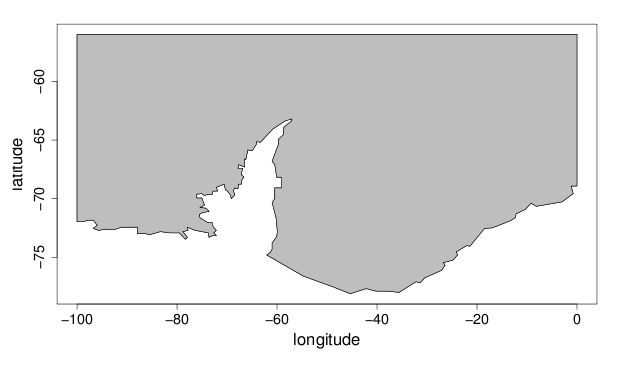
\includegraphics[width=2.5in]{figs/peninsula.png}
       \ec
\end{frame}

\begin{frame}
	\frametitle{Leakage (or, ``whales don't live in glaciers'')}
       \bi
         \item Smoothing of complex domains makes this a lot more difficult.
         \item Problem of leakage.
         \item Wrong metric.
         \item Euclidean distance doesn't always make sense.
       \ei
       \bc\begin{tabular}{@{}cc}
          & \\
          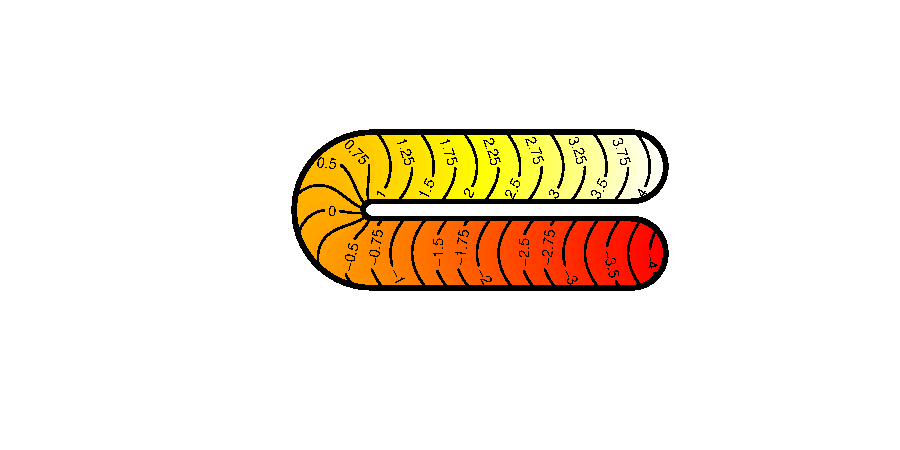
\includegraphics[width=2in, trim=1in 1in 1in 1in]{figs/ramsayhorseshoe} & 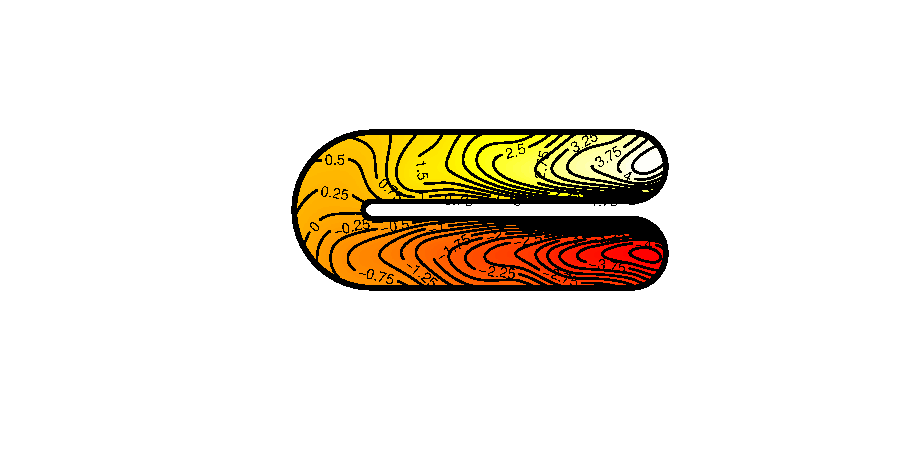
\includegraphics[width=2in, trim=1in 1in 1in 1in]{figs/leakageexample}\\
          (modified) Ramsay test function & Thin plate spline fit\\
       \end{tabular}\ec
\end{frame}

\subsection{Smoothing with splines}

\begin{frame}
	\frametitle{Smoothing with penalties}
      \bi
        \item Do smoothing with splines in an additive model framework.
        \item Take some linear combination of (known) basis functions.
        \item Penalize based on integral of second squared derivative:
        \ei
            \begin{equation*}
	            \int\int_{\mathbf{R}^2} \Big( \Big(\frac{\partial^2 f(x_1,x_2)}{\partial x_1^2}\Big)^2 + \Big(\frac{\partial^2 f(x_1,x_2)}{\partial x_1 \partial x_2}\Big)^2 + \Big(\frac{\partial^2 f(x_1,x_2)}{\partial x_2^2}\Big)^2\Big) \text{d}x_1\text{d}x_2.
            \end{equation*}
      \bi
        \item Using thin plate regression splines (eg Wood (2003)).
        \includegraphics[width=4in]{figs/tprsex} 
      \ei
\end{frame}

%%%%%%%%%%%%%%%%%%%%%%%%%%%%%%%%%%

\subsection{Solutions}

\begin{frame}
	\frametitle{Proposed solutions to leakage problems}
	Two categories: PDE boundary condition based, within-area distance based.
       \bi
         \item PDEs:
	  \bi
             \item FELSPLINE (Ramsay, 2002).
             \item Soap film smoothers (Wood \emph{et al}, 2008).
           \ei
           \item Within-area distance
           \bi
             \item Geodesic Low-Rank  Thin Plate Splines (GLTPS) (Wang and Ranalli, 2007).
           \ei
        \ei
        \bc\begin{tabular}{@{}cc}
          & \\
        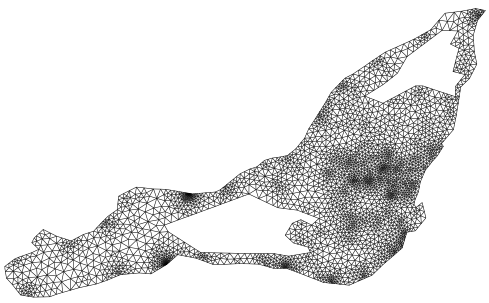
\includegraphics[width=2in]{figs/ramsaytriangulation.png}&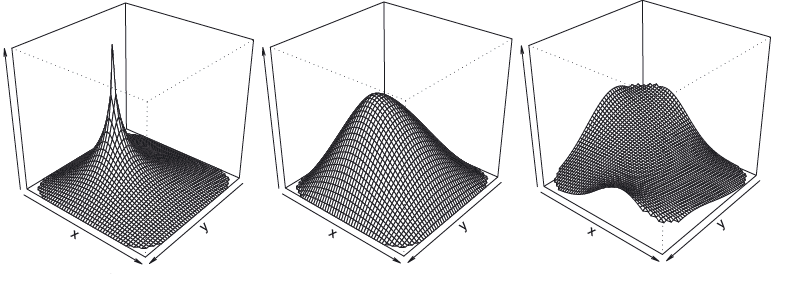
\includegraphics[width=2in]{figs/soapbases.png}\\
        \end{tabular}
        \ec
\end{frame}

%\begin{frame}
%	\frametitle{Explanation of FELSPLINE/soap/GLTPS}
%\end{frame}

\begin{frame}
	\frametitle{``The Third Way''}
      \bi
         \item Domain morphing - think of domain as silly putty.
         \item Takes into account within-area distance.
         \item Potentially less computationally intensive. 
         \item Eilers (2006) proposes Schwarz-Christoffel transform.
         \item Gives a known domain - easier to smooth over.
      \ei
      \bc
         \textbf{However:}
      \ec
      \bi
         \item Crowding - numerical singularities.
         \item Not clear what this does to the smoothness penalty - artefacts, penalty issues - but NOT GOOD!
      \ei
      \bc
         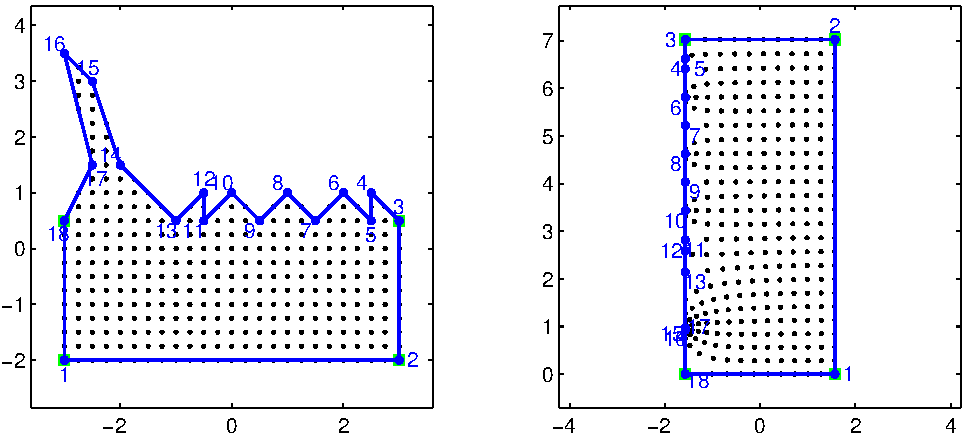
\includegraphics[height=1in]{figs/matlab-test-3}
      \ec
\end{frame}



\section{Multidimensional Scaling}

\subsection{Details}

\begin{frame}
	\frametitle{Multidimensional scaling and within-area distances}
       \bi
         \item Idea: use MDS to arrange points in the domain according to their distance within the domain.
         \ei
         \bc \textbf{Scheme:} \ec
         \bi
         \item First need to find the within-area distances.
         \item Perform MDS on the matrix of within-area distances.
         \item Find the new configuration of the points.
         \item Smooth over the new points.
        \ei
\end{frame}

\begin{frame}
	\frametitle{Multidimensional scaling refresher}
       \bi
         \item Use double centred matrix of between point distances, $D$, using the eigen-decomposition of $DD^T$ we can find new points.
         \item Finds a projection of points such that Euclidean distance between points in new arrangement is approximately the same as the distances in $D$.
          \item New points can be added into the MDS configuration via Gower's interpolation (Gower, 1968)
        \ei
            \centering
            % this is just generated from wt2-test.R
              \includegraphics[width=3in]{figs/wt2-coloured.pdf}\\
        
\end{frame}

\subsection{Finding the within-area distances}

\begin{frame}
	\frametitle{A ``new'' algorithm for finding within-area distances}

	\bc \textbf{So, how do we find the distances to put in D?}\ec
\end{frame}

\begin{frame}
	\frametitle{Finding the path - 1}
            \centering
             % trim order l b r t
              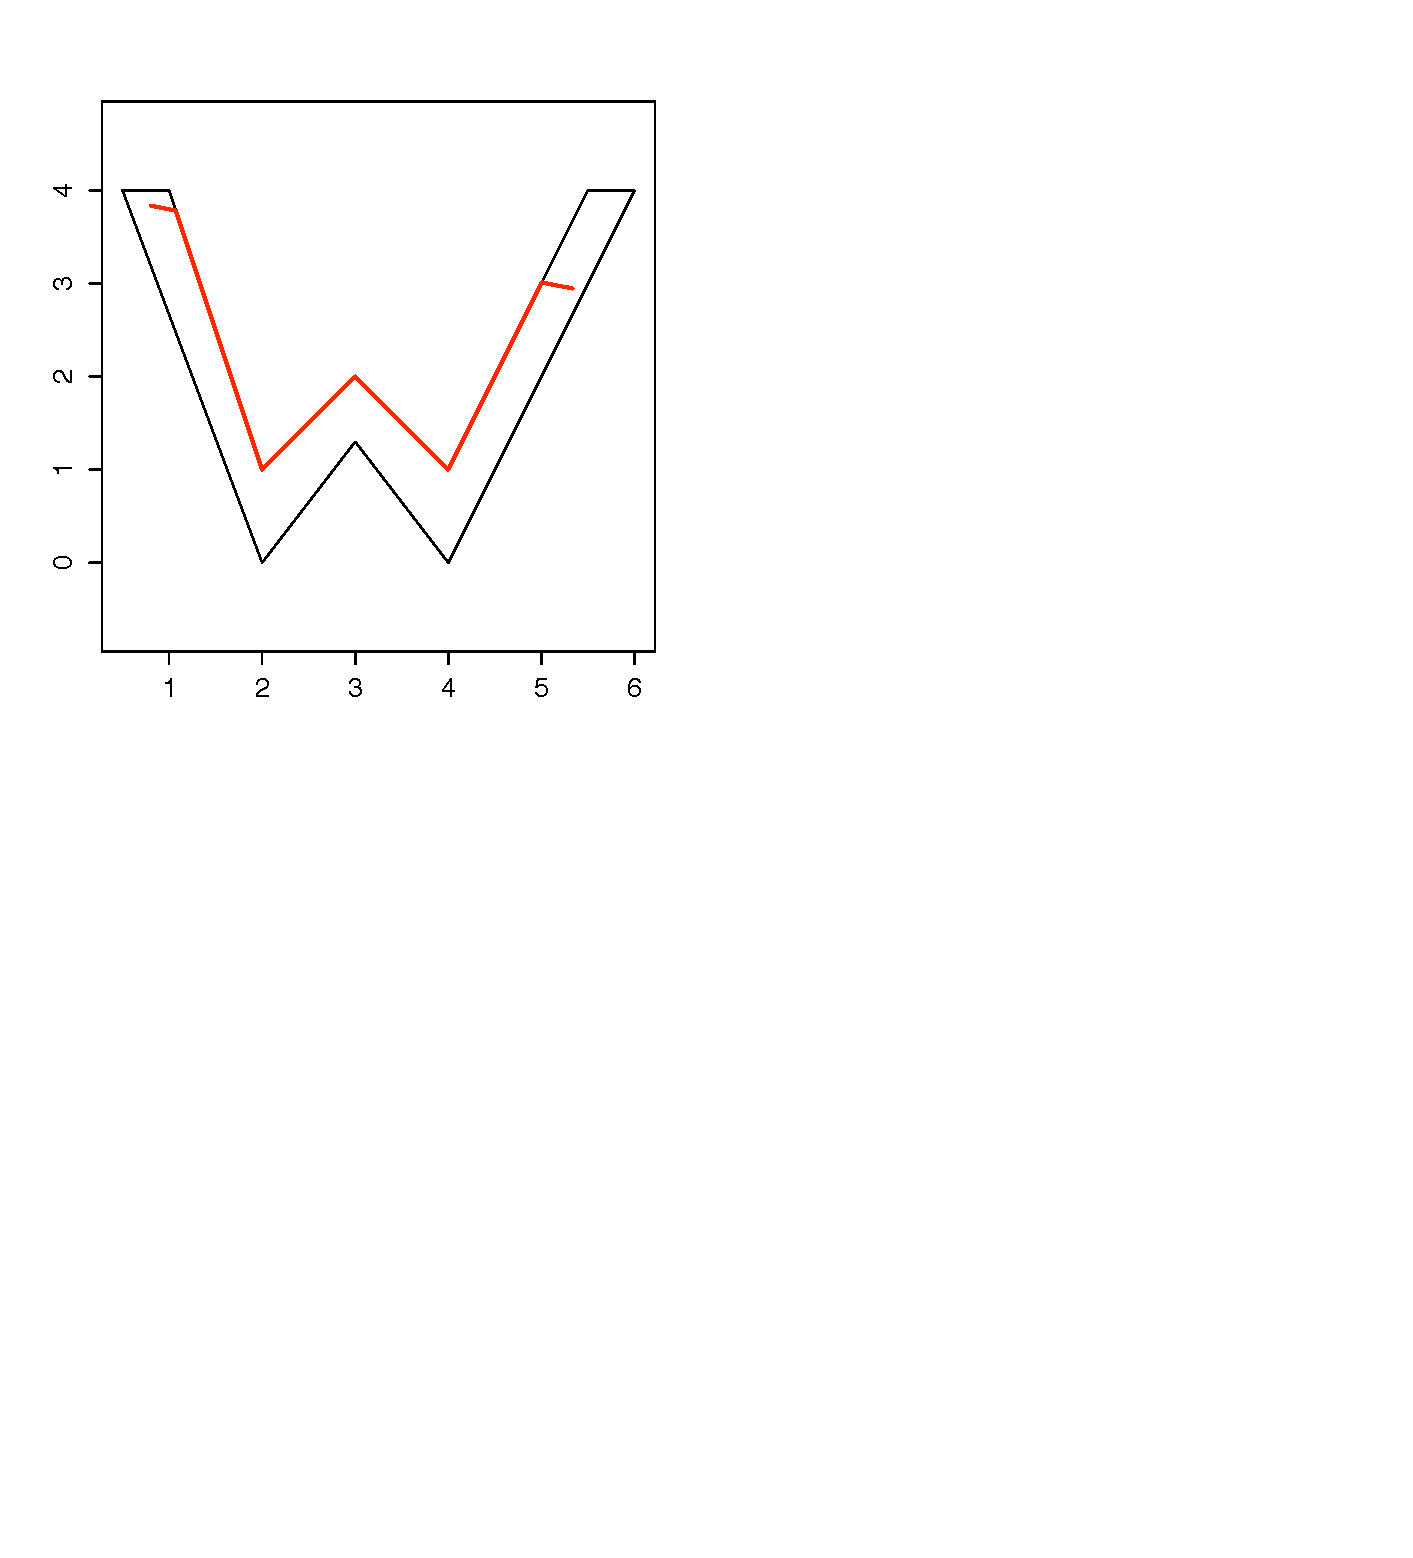
\includegraphics[width=2.75in]{figs/wood-2}\\
\end{frame}

\begin{frame}
	\frametitle{Finding the path - 2}
            \centering
              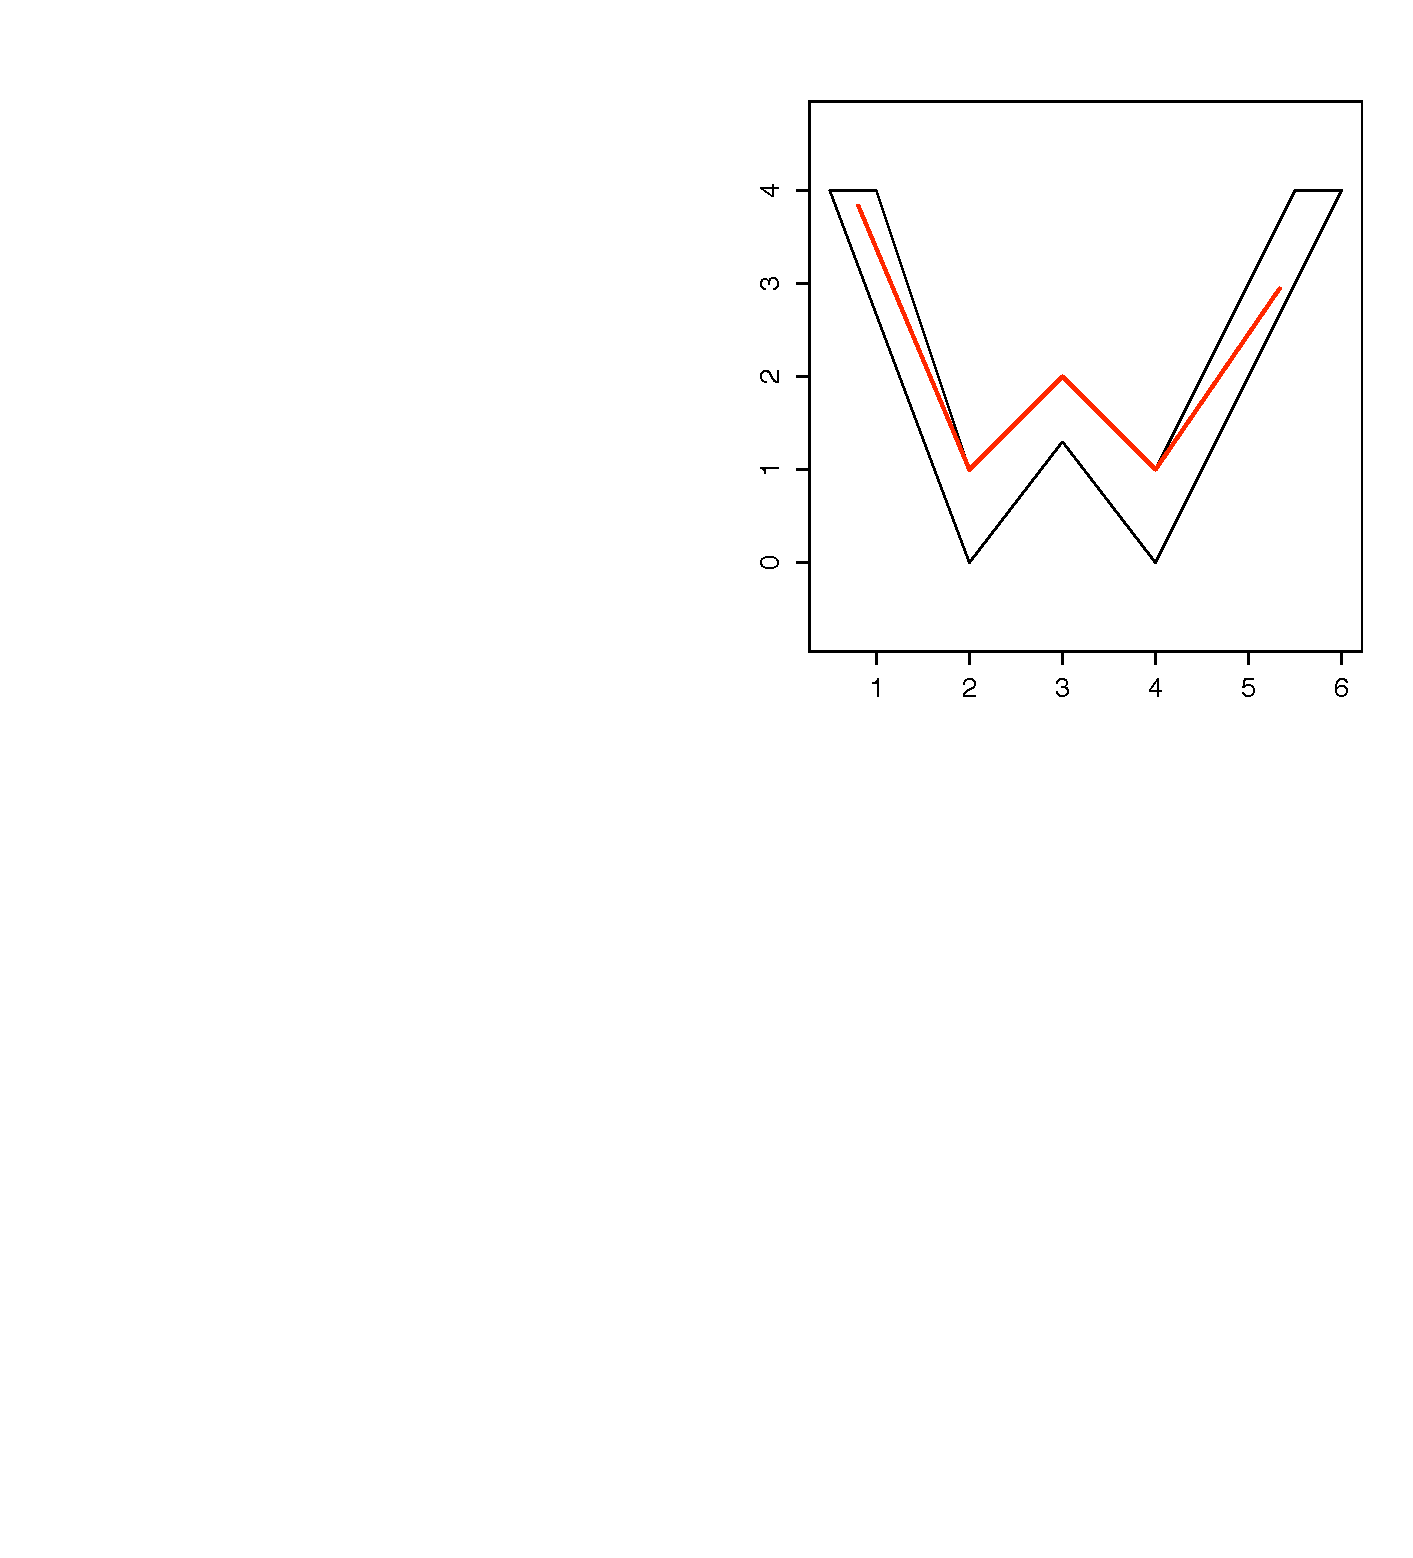
\includegraphics[width=2.75in]{figs/wood-1}\\
\end{frame}

\begin{frame}
	\frametitle{Finding the path - 3}
            \centering
              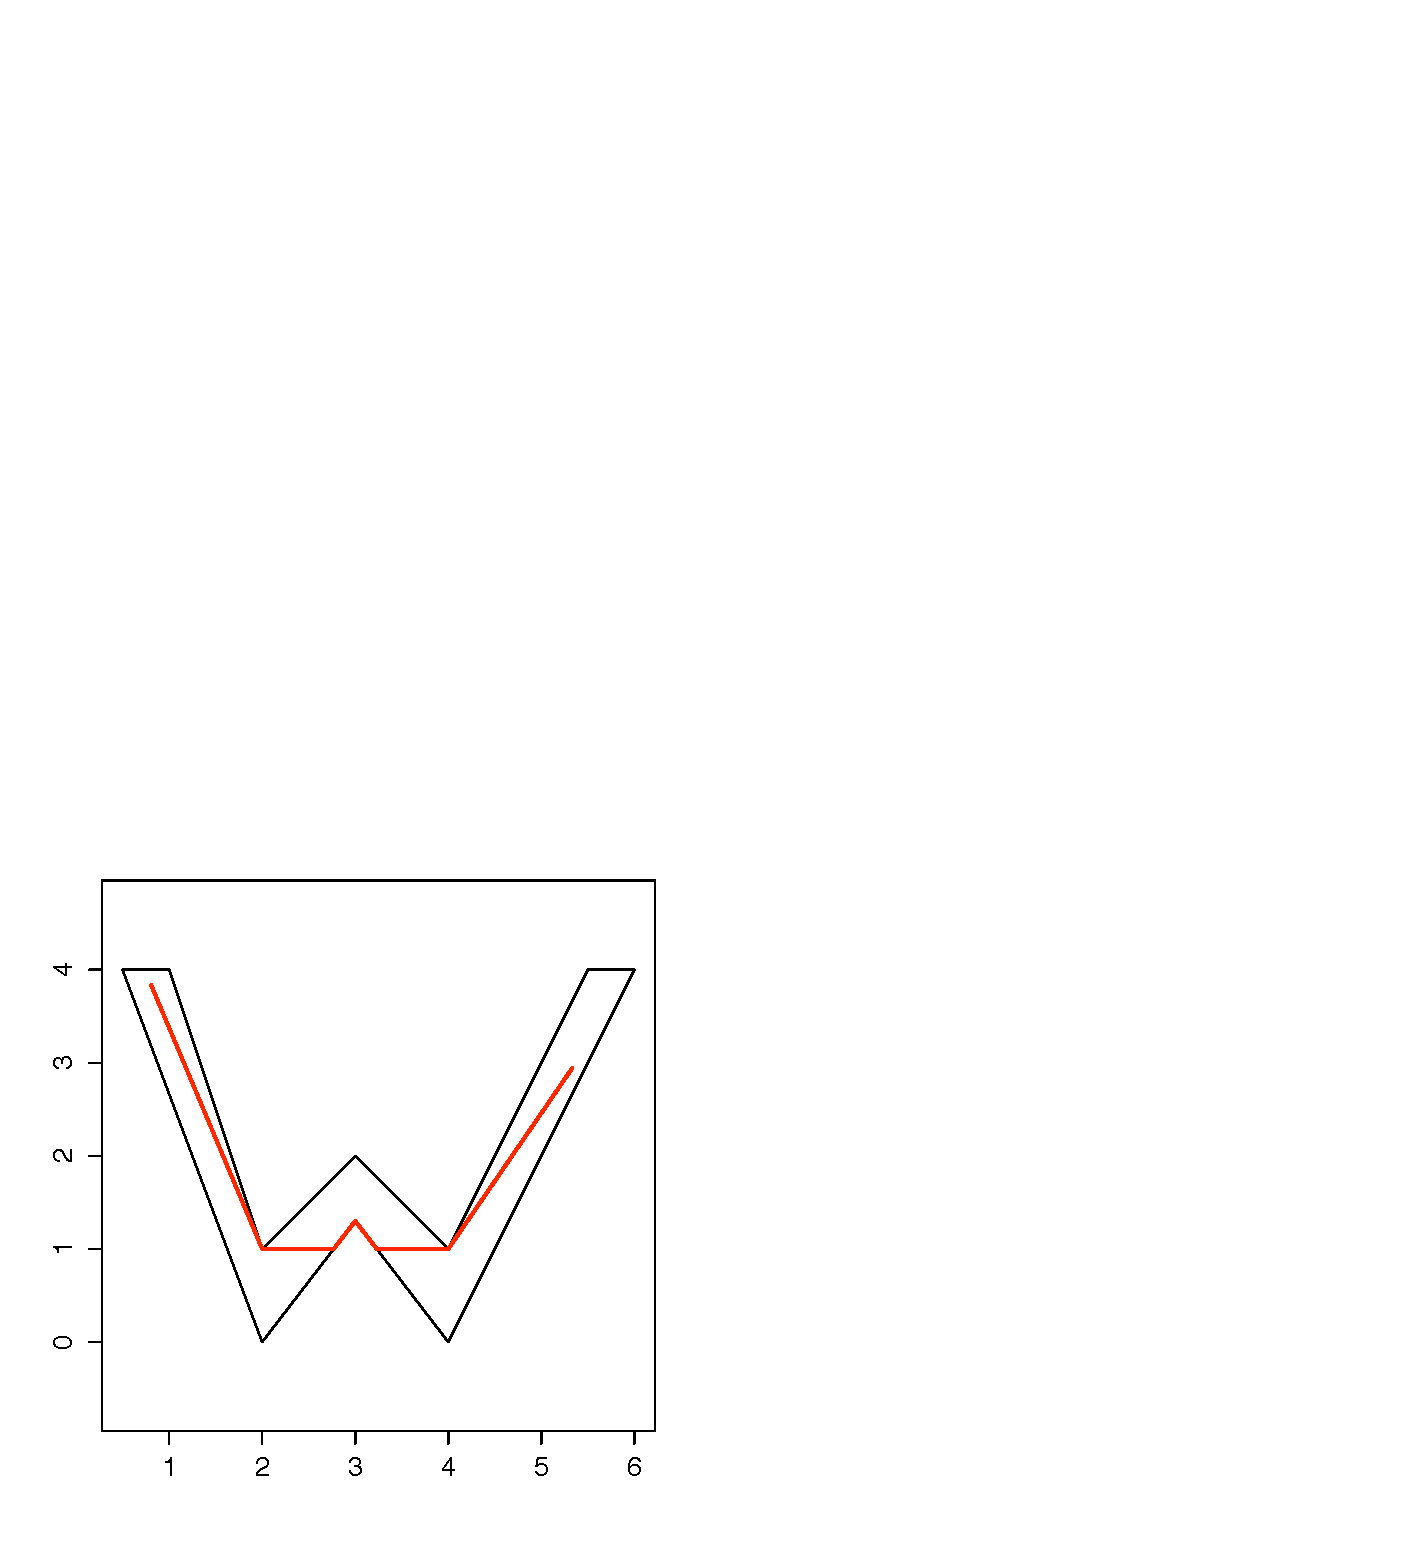
\includegraphics[width=2.75in]{figs/wood-3}\\
\end{frame}

\begin{frame}
	\frametitle{Finding the path - 4}
            \centering
              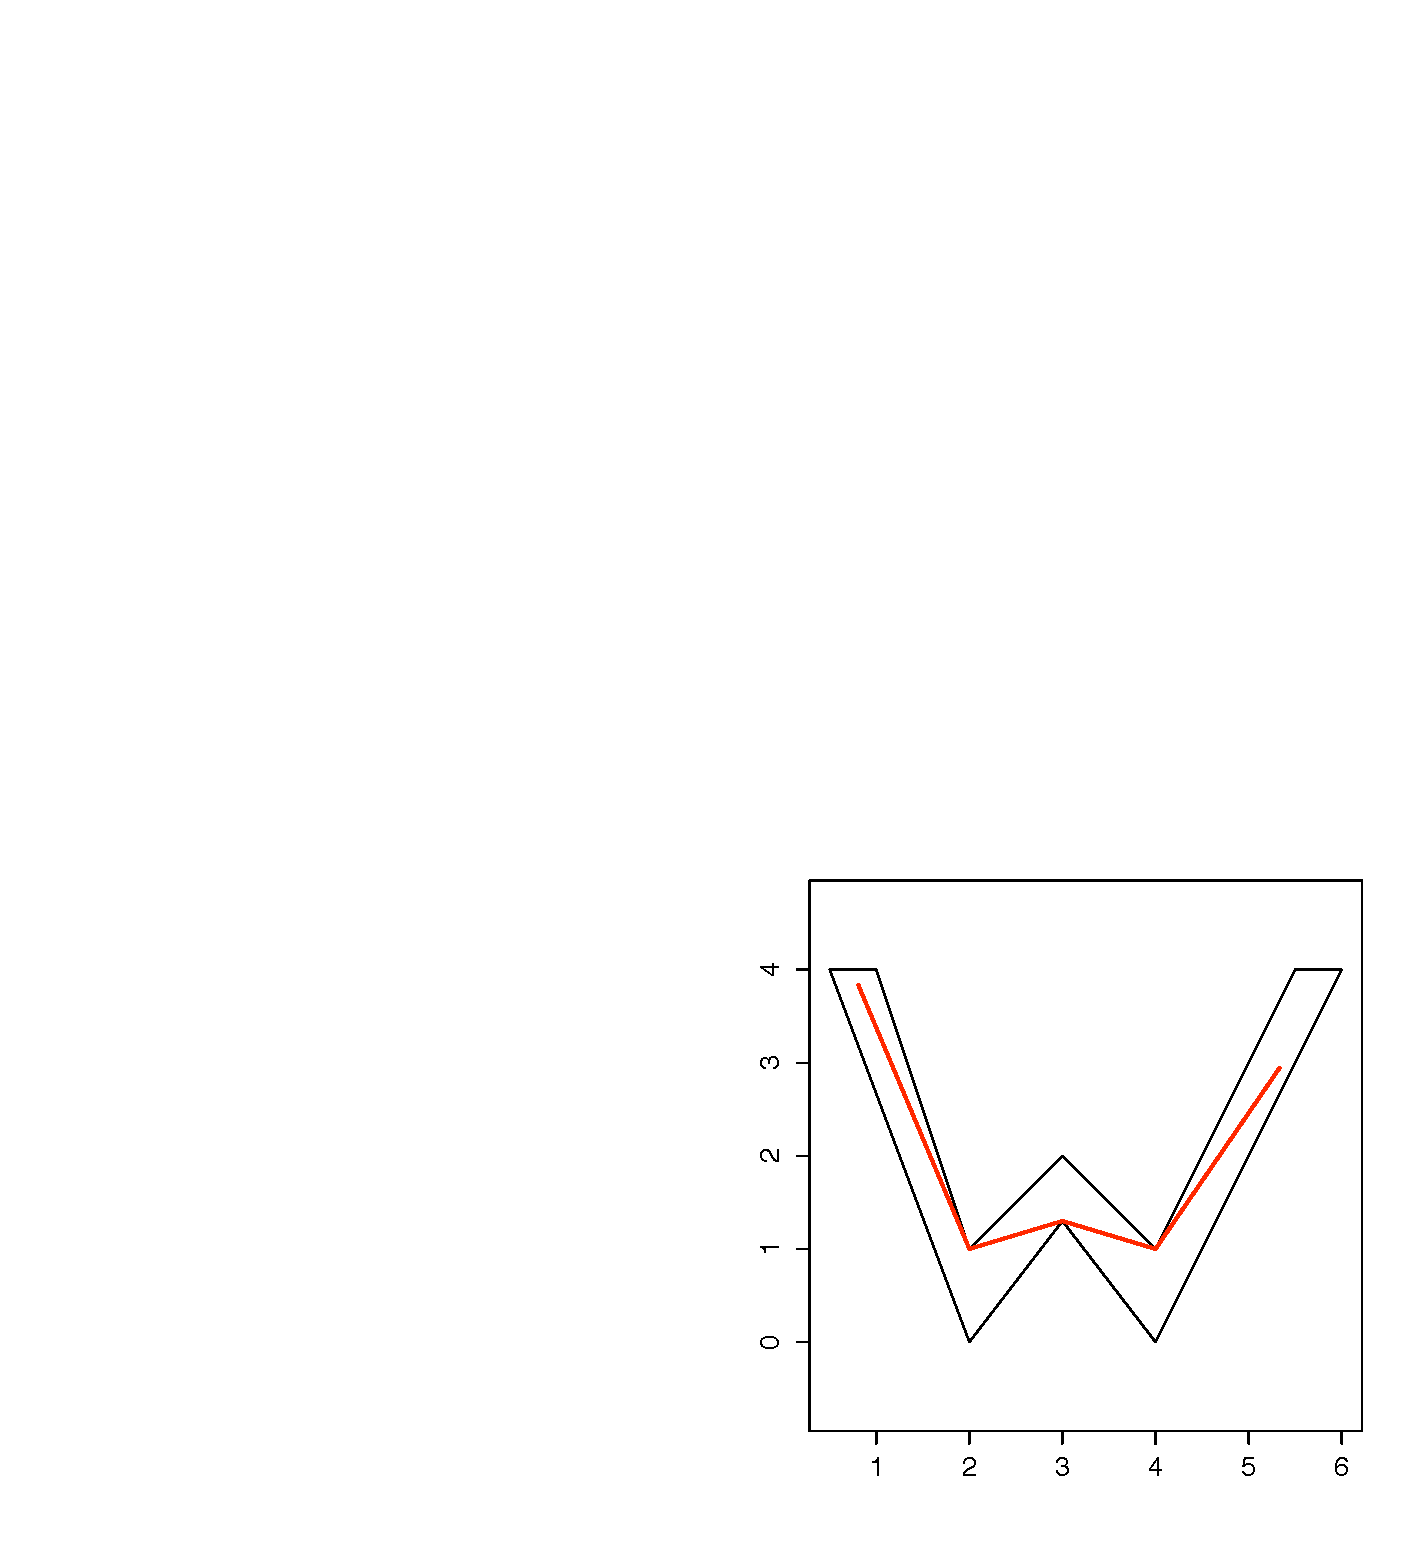
\includegraphics[width=2.75in]{figs/wood-4}\\
\end{frame}

\subsection{Simulation Results}

\begin{frame}
	\frametitle{Simulations}
	\bc \textbf{But how does it perform?}\ec
\end{frame}


\begin{frame}
	\frametitle{Ramsay simulations}
            \centering
              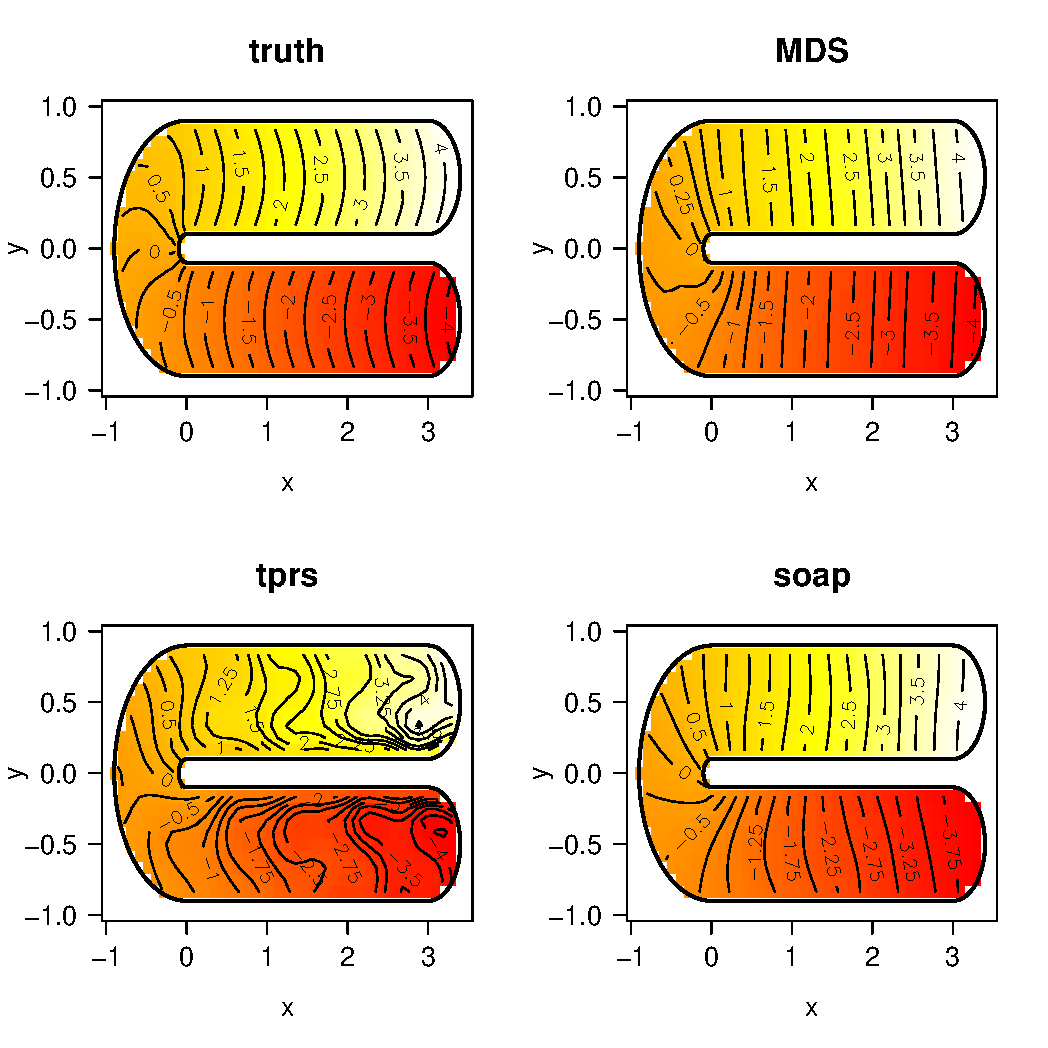
\includegraphics[width=4in]{figs/ramsay-low.pdf}\\
\end{frame}

\begin{frame}
	\frametitle{The Aral sea}
	\textbf{ARAL SEA PICTURE}
\end{frame}

\begin{frame}
	\frametitle{The Aral sea}
            \centering
              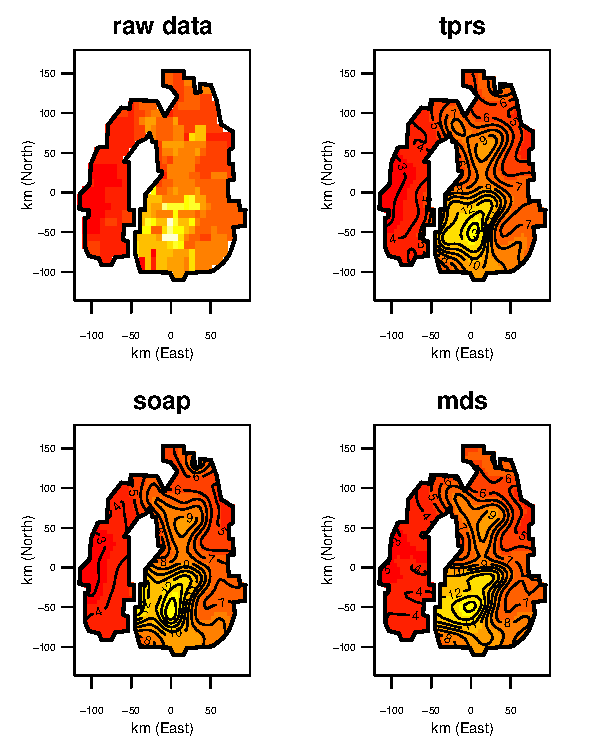
\includegraphics[height=3.5in]{figs/aral-fit.pdf}\\
\end{frame}

\begin{frame}
	\frametitle{But...}
          \bi
            \item Computationally costly to find the within-area distances. (Esp. prediction.)
            \item Comparative in MSE terms to the soap film smoother.
            \item Artefacts -- ordering?
            \item Taking a $m$-D projection of $n$-D space.
           \ei
	\textbf{[[3D PLOT]]}
	\begin{figure}
	         	\centering
              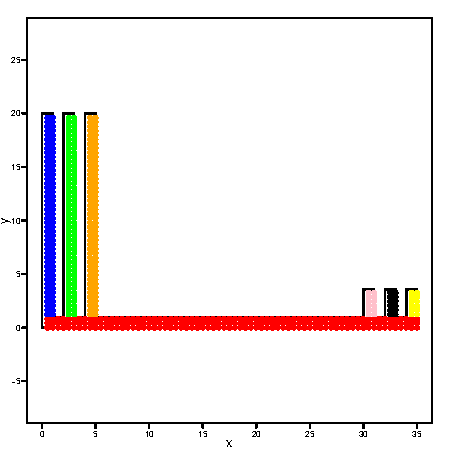
\includegraphics[height=1.75in]{figs/comb.pdf} 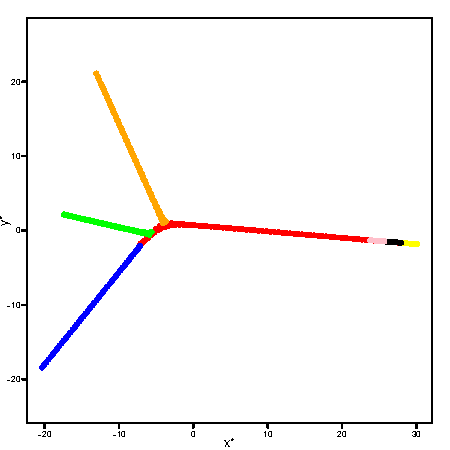
\includegraphics[height=1.75in]{figs/comb-2d.pdf}
	\end{figure}
\end{frame}



\begin{frame}
	\frametitle{Ordering}
	\bi
		\item So, where are the artefacts coming from?
		\item Taking projections of $n$-dimensional space.
		\item Points can lose ordering.
		\item 3-D projection does better, but can we keep going? (Nullspace gets BIG!)
	\ei
\end{frame}

%%%%%%%%%%%%%%%%%%%%%%%%%%%%%%%%%

\section{High dimensional smoothing with Duchon splines}

\begin{frame}
	\frametitle{High dimensional smoothing with Duchon splines}
	\bc \textbf{How can we fix this?}\ec
\end{frame}



\subsection{Nullspaces}

%% say something about radial functions + ``planes''
\begin{frame}
	\frametitle{Nullspaces}
	\bi
		\item TPRS functions of the form:
		\begin{align*}
		f(\mathbf{x}) &= \sum_{i=1}^n \delta_i \eta_{md}(\mathbf{x}-\mathbf{x_i}) + \sum_{j=1}^M \alpha_j \phi_j(\mathbf{x})\\
		&= \text{radial basis functions} + \text{``planes''}
		\end{align*}
		\item $\phi_j(\mathbf{x})$ are linearly independent polynomials of degree $< m$.
	\ei
	\textbf{WHAT IS $m$, $d$ etc!!!}
\end{frame}


% why high dimensions are bad in tprs
%	diagram of nullspace sizes
\begin{frame}
	\frametitle{When nullspaces get big...(I)}
	\bi
		\item For TPRS, nullspace size is 
		\begin{equation*}
			M=\begin{pmatrix} m+d-1 \\ d  \end{pmatrix}
		\end{equation*}
		Where \begin{align*}
				m &= \text{the derivative order in the penalty}\\
				d &= \text{smoothing dimension}
			\end{align*}
		\item \textbf{AND} must obey $2m>d$ \\smoothing dimension++ $\Rightarrow$ derivative order++++.
		\item $M$ gets very big, very fast.
	\ei
\end{frame}

\begin{frame}
	\frametitle{When nullspaces get big... (II)}
	\begin{figure}
	\centering
			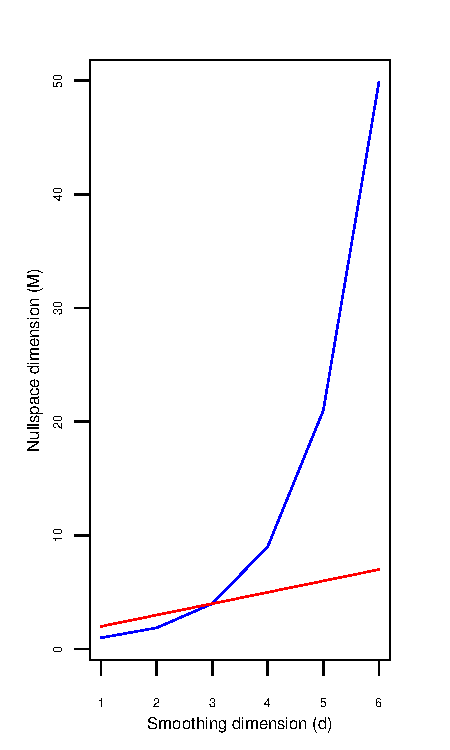
\includegraphics[height=3.4in]{figs/nullspace-dim.pdf} 
	\end{figure}
\end{frame}

\begin{frame}
	\frametitle{A brief digression into Fourier transforms (I)} 
	\bi
		\item Given some function, we can take the Fourier transform:
		\begin{equation*}
			\mathfrak{F} g(\boldsymbol{\tau}) = \int \ldots \int_{\mathbb{R}^n} e^{2 \pi \sqrt{-1} \mathbf{x}^\text{T} \boldsymbol{\tau}} g(\mathbf{x}) \text{d}\mathbf{x}.
		\end{equation*}
		\item Can think of this as a change of basis \textbf{OR} as decomposing the function into frequency components.	
	\ei
\textbf{THINK ABOUT THIS!!!}
\end{frame}

%\begin{frame}
%	\frametitle{A brief digression into Fourier transforms (II)} 
%	\bi
%		\item 
%	\ei
%\end{frame}



% digression into Fourier transforms

% build up to Duchon splines
%	diagram of nullspace sizes
% talk about manifolds

\subsection{Duchon splines}

\begin{frame}
	\frametitle{Enter Jean Duchon...} 
	\begin{figure}
		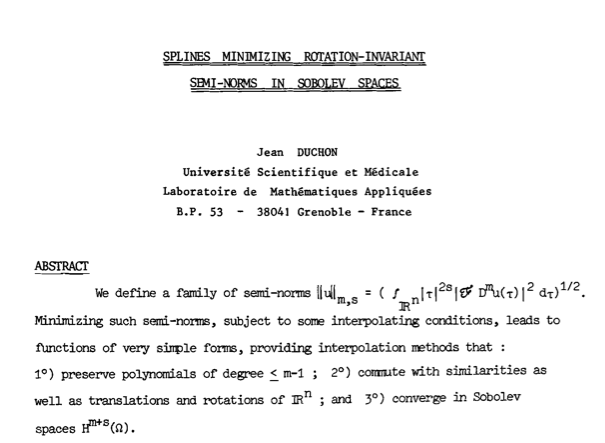
\includegraphics[height=3in]{figs/Duchon-paper.png}
	\end{figure}

\end{frame}

\begin{frame}
	\frametitle{High dimensional smoothing with Duchon splines}
	Wood (2003) type penalty:
	\begin{equation*}
		J_{m,d} = \int \ldots \int_{\mathbb{R}^d} \sum_{\nu_1 + \dots + \nu_d=m} \frac{m!}{\nu_1! \dots \nu_d!}\Big( \frac{\partial^m f(x_1,\dots,x_d)}{\partial x_1^{\nu_1} \ldots  \partial x_d^{\nu_d}} \Big)^2 \text{d} x_1 \ldots  \text{d} x_d
	\end{equation*}
	Why not take the Fourier transform? (Equivalent by Plancherel theorem)
	\begin{equation*}
		\breve{J}_{m,d} = \int \ldots \int_{\mathbb{R}^d} \sum_{\nu_1 + \dots + \nu_d=m} \frac{m!}{\nu_1! \dots \nu_d!}\Big( \mathfrak{F} \frac{\partial^m f}{\partial x_1^{\nu_1} \ldots  \partial x_d^{\nu_d}}(\boldsymbol{\tau}) \Big)^2 \text{d} \boldsymbol{\tau}
	\end{equation*}
	Putting in some arbitrary weighting, $w(\boldsymbol{\tau})$:
	\begin{equation*}
		\breve{J}_{m,d} = \int \ldots \int_{\mathbb{R}^d} w(\boldsymbol{\tau}) \sum_{\nu_1 + \dots + \nu_d=m} \frac{m!}{\nu_1! \dots \nu_d!}\Big( \mathfrak{F} \frac{\partial^m f}{\partial x_1^{\nu_1} \ldots  \partial x_d^{\nu_d}}(\boldsymbol{\tau}) \Big)^2 \text{d} \boldsymbol{\tau}
	\end{equation*}
\end{frame}

\begin{frame}
	\frametitle{Duchon splines penalty}
	Let $w(\boldsymbol{\tau})=\lvert \boldsymbol{\tau} \rvert^{2s}$ (Duchon 1977)
	\begin{equation*}
		\breve{J}_{m,d} = \int \ldots \int_{\mathbb{R}^n} \lvert \boldsymbol{\tau} \rvert^{2s} \sum_{\nu_1 + \dots + \nu_d=m} \frac{m!}{\nu_1! \dots \nu_d!}\Big( \mathfrak{F} \frac{\partial^m f}{\partial x_1^{\nu_1} \ldots  \partial x_d^{\nu_d}}(\boldsymbol{\tau}) \Big)^2 \text{d} \boldsymbol{\tau}
	\end{equation*}	
	
	\bi
	\item This penalises high frequency components of the derivatives.
	\item Now the condition relating $d$ and $m$ is $d/2 -m \leq s$.
	\item Given we want to use $m=2$ (some pseudo-theoretical reasons for that) and we have a set $d$, determine $s$ by
	\begin{equation}
		s=d/2-2
	\end{equation}
	\ei
\end{frame}

% using ml/gcv
\begin{frame}
	\frametitle{Using ML/GCV score to select projection dimension}
   \bi
      \item So, we can now smooth in higher dimensions, \textbf{but how many?}
      \item Select MDS dimension using GCV or ML score.
      \item Fit model in a range of dimensions, pick best score.
      \item No monotonicity guarantees.
      % FIGURE OF SCORE VS DIM HERE
   \ei
\end{frame}



\subsection{Results}

% some results
\begin{frame}
	\frametitle{Pretend coastline}
	\begin{figure}
	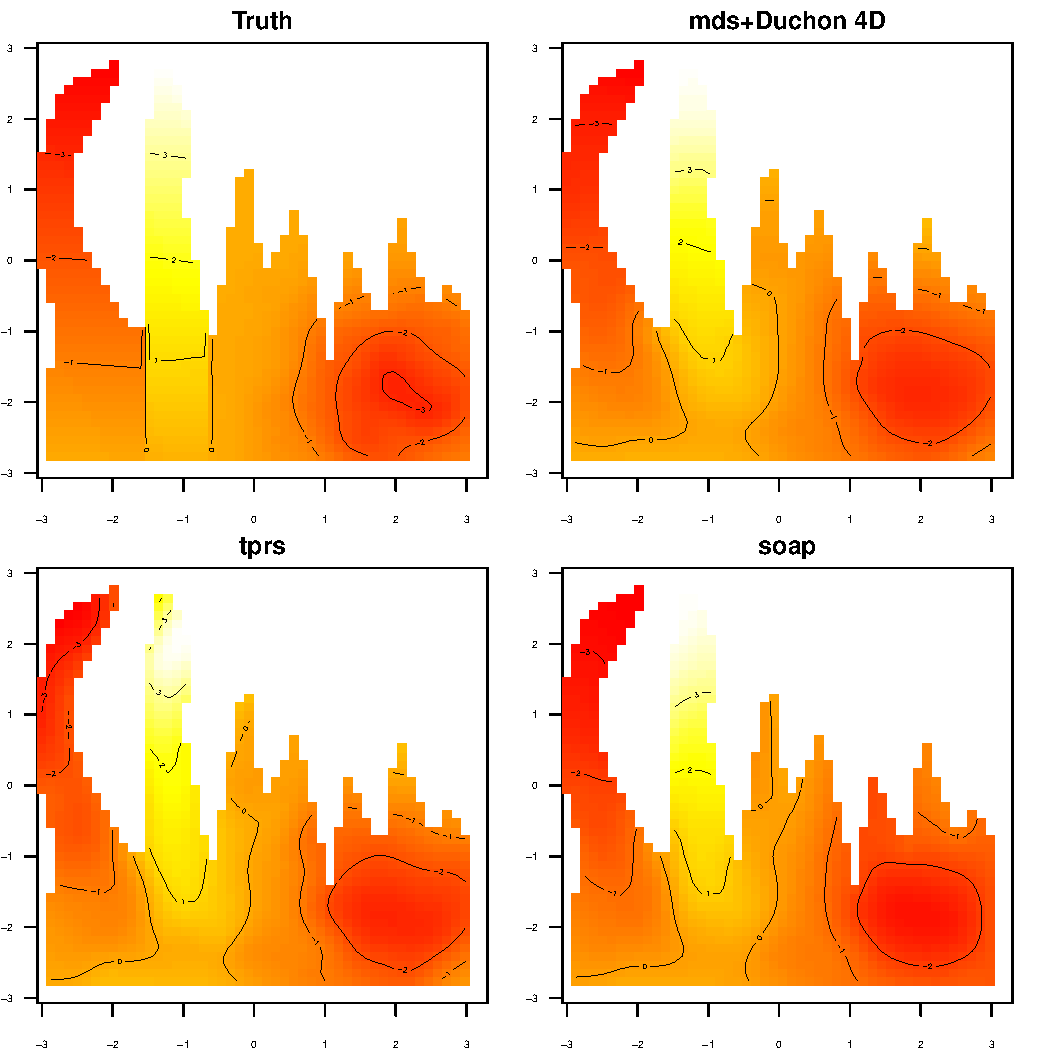
\includegraphics[height=3.25in]{figs/wt2-comp.pdf}
	\end{figure}
\end{frame}

\begin{frame}
	\frametitle{Aral sea}
   \begin{figure}
      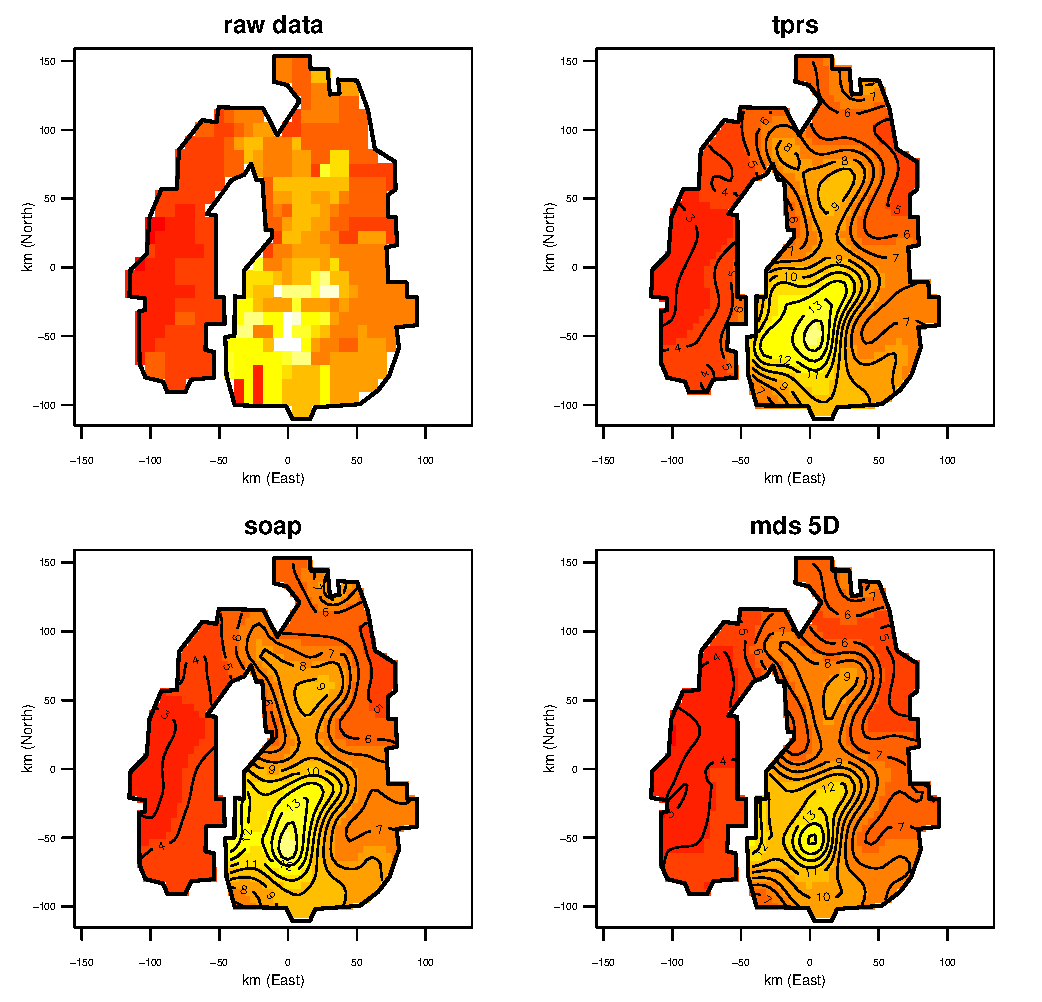
\includegraphics[height=3.5in]{figs/aral-duchon-comp.pdf}
   \end{figure}
\end{frame}

%\begin{frame}
%	\frametitle{Something something something}
%\end{frame}

%\begin{frame}
%	\frametitle{}
%\end{frame}


%%%%%%%%%%%%%%%%%%%%%%%%%%%%%%%%%%%%%%%%
% General distance stuff
\section{General distance smoothing}

\begin{frame}
	\frametitle{General distance smoothing}
	\bi
		\item Given a general distance matrix, $D$.
		\item Project the points in $D$ using MDS.
		\item Smooth over those points.
	\ei
	\centering Examples:
	\bi
		\item Voting data
		\item Microarrays
		\item Socio-economic variables
	\ei	
\end{frame}

% EXAMPLES
%	SHOW MP DATA PLOT?


%%%%%%%%%%%%%% RE-WRITE THIS!!!!
\section{Conclusions}

\begin{frame}
	\frametitle{Final comments}
          \bi
            \item Something
            \item Something
            \item Something
           \ei
\end{frame}

\begin{frame}
	\frametitle{References}
       \bi
         \item T. Ramsay. \emph{Spline smoothing over difficult regions. JRSSB, 2002}
         \item P.H.C. Eilers. \emph{P-spline smoothing on difficult domains. University of Munich seminar, 2006}
	\item J.C. Gower. \emph{Adding a point to vector diagrams in multivariate analysis. Biometrika, 1968.}
	\item Duchon, J. (1977). \emph{Splines minimizing rotation-invariant semi-norms in Sobolev spaces. Constructive theory of functions of several variables.} Springer.
        \ei
        Slides available at \url{http://people.bath.ac.uk/dlm27}
\end{frame}

\begin{frame}
	\frametitle{Appendix - Ordering problems in 4-D}
	\centering
            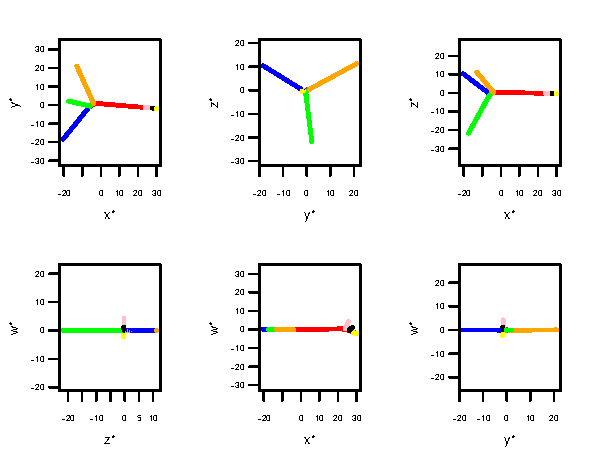
\includegraphics[height=3in]{figs/comb-4d.pdf}	
\end{frame}

\begin{frame}
	\frametitle{Appendix - A ``new'' algorithm for finding within-area distances}
	\bi
		\item Algorithm ``bounces'' around inside the polygon.
		\item Initial path is just the path around the edge, then iterate over two steps: \textit{delete} and \textit{alter}.
		\item Delete (iterating over all nodes):
			\bi \item If we can shorten the path by simply deleting a node, do that.
			\ei
		\item Alter (iterating over all nodes):
			\bi \item If we can find a shorter sub-path by bouncing off the other ``side'' of the polygon, do that.
			\ei
	\ei
\end{frame}


\end{document}
